\documentclass[12pt,oneside]{article}
\usepackage{light}
\newcommand{\mfigure}[3]{\bigskip\centerline{\resizebox{#1}{#2}{\includegraphics{#3}}}\bigskip}
\newcommand{\hint}[1]{({\it Hint: #1})}
\newcommand{\brule}[1]{\underline{\hspace{#1}}}
\newcommand{\ang}[1]{\left< #1 \right>}
\newcommand{\beats}{\rightarrow}

\newenvironment{falseproof}
{\begin{proof}[False proof]}
{\end{proof}}

\hidesolutions
\showsolutions

\begin{document}
\generic{Midterm Practice Problems}{October 19, 2016}

\instatements{
\vspace{24pt}
\textbf{Name:} \rule{5in}{0.5pt}

\begin{itemize}

\item This quiz is \textbf{closed book}, but you may have one $8.5
\times 11$'' sheet with notes in your own handwriting on both sides.

\item Calculators and electronic devices are not allowed.

\item You may assume all of the results presented in class.

\item Please show your work.  Partial credit cannot be given for a wrong
answer if your work isn't shown.

\item Write your solutions in the space provided.  If you
need more space, write on the back of the sheet containing the
problem.  Please keep your entire answer to a problem on that
problem's page.

\item Be neat and write legibly.  You will be graded not only on the
correctness of your answers, but also on the clarity with which you
express them.

\item If you get stuck on a problem, move on to others. The problems 
are not arranged in order of difficulty.

\end{itemize}

\vspace{0.25in}

%\begin{center}
%{\large
%\begin{tabular}{|c|c|c|c|}
%\hline
%Problem & Points & Grade & Grader \\ \hline \hline
%1 & 10 & & \\ \hline
%2 & 15 & & \\ \hline
%3 & 20 & & \\ \hline
%4 & 10 & & \\ \hline
%5 & 15 & & \\ \hline
%6 & 10 & & \\ \hline
%7 & 20 & & \\ \hline
%Total & 100 & & \\ \hline
%\end{tabular}
%}
%\end{center}
}
\instatements{\newpage}

\begin{problem}{12}
Let $X$ be the set of students in 6.042. Let $Y$ be the set of problems on this quiz. For $x \in X$ and $y \in Y$, let $P(x,y)$ be the statement ``Student $x$ got full points on problem $y$''. Let $Q(x)$ be the statement ``Student $x$ drops 6.042''.
\bparts
\ppart{6}
Convert the following statements into English.
\begin{enumerate}
\item $(\exists x\in X, Q(x) ) \Rightarrow (\forall x\in X, Q(x))$.

\solution{If a student in 6.042 drops the class, then all the students in 6.042
will drop the class.}
%\vspace{2in}
\item $\forall x\in X ((\exists y\in Y \neg P(x,y)) \Rightarrow  Q(x))$

\solution{For every student in 6.042, if there is a problem on the quiz 
that he / she doesn't get full points on, he / she will drop the class.}
%\vspace{2in}
\item $\exists x\in X (\neg Q(x))$.

\solution{There is a student in 6.042 who won't drop the class.}
%\vspace{2in}
\end{enumerate}
\ppart {6}
Assuming 1,2 and 3 are true, what can you say about your score on this quiz?

\solution{I will get full points on the quiz.}

\eparts

\end{problem}


%%%%%%%%%%%%%%%%%%%%%%%%%%%%%%%%%%%%%%%%%%%%%%%%%%%%%%%%%%%%%%%%%%%%%%%%%

\newpage

\begin{problem}{20}
6 people are sitting in a circle. Each person has a number.
They do a ritual during each round that makes their numbers update.
Each person, to get his number for round $n+1$, takes his number from round $n$, then adds his right neighbor's number from round $n$ to it, and then subtracts his left neighbor's number from round $n$ from it. 

For example if on the current round there is a person $A$ whose number is 5, and $A$'s right neighbor's number is 4, and $A$'s left neighbor's number is 6, then in the following round, $A$'s number will be $5 + 4 - 6  = 3$.

Initially the people are given the numbers $1,2,3,4,5,6$ (in clockwise order, and the person with $6$ is sitting next to the person with $1$).

Thus, after 1 round, their numbers will be $5, 0, 1, 2, 3, 10$.

Prove that there will never be a round when all their numbers are equal.

BIG HINT: Consider what happens to the sum of the numbers.

\solution{
\begin{lemma}
After every round, each number is an integer,
and the sum of the numbers is 21.
\end{lemma}
\begin{proof}
The inductive hypothesis $P(n)$ states that after round $n$, the
sum of the numbers is 21 and all numbers are integers.

The base case $P(0)$ follows from summing up the values of
the initial settings of the numbers and noting that all initial values are
integers.

Assuming that $P(n)$ holds, we show that $P(n+1)$ holds.  
Let the values of the numbers at round $n$ be $a_1,\ldots,a_6$.
For each $i$, the new value of the $i^{th}$ person is $a_i +a_{i+1 \rem 6} - a_{i-1 \rem 6}$.
Since the inductive hypothesis tells us that
$a_i,a_{i+1 \rem 6}$ and $a_{i-1 \rem 6}$ are all integers, the new value
of the $i^{th}$ person is also an integer.
The sum at round $n+1$ is $$\sum_{1 \leq i \leq 6} a_i +a_{i+1 \rem 6} - a_{i-1 \rem 6}
= \sum_{1 \leq i \leq 6} a_i + a_i - a_i  = \sum_{1 \leq i \leq 6} a_i =21.$$
The second equality is by reordering the summation, and the third equality
is from the inductive hypothesis.
And so $P(n+1)$ holds by the principle of induction.
\end{proof}

Assume for the purposes of contradiction that there is a round
in which all numbers
are equal to the value $v$.  By the lemma, $v=21/6$ and $v$ is
an integer, which is impossible since 6 does not divide $21$.
Thus, there cannot be a round in which all numbers are equal.
}
\end{problem}


%%%%%%%%%%%%%%%%%%%%%%%%%%%%%%%%%%%%%%%%%%%%%%%%%%%%%%%%%%%%%%%%%%%%%
% taken from: new problem
% comments: strong induction and number theory
%
\newpage
\begin{problem}{15}
We define the sequence of numbers
\begin{eqnarray*}
a_n = \begin{cases}
  1                                    &  \text{if $0 \leq n \leq 3$,}\\
  a_{n-1} + a_{n-2} + a_{n-3}+ a_{n-4} &  \text{if $n \geq 4$.}
 \end{cases}
\end{eqnarray*}

Prove that $a_n \equiv 1 \pmod{3}$ for all $n\geq 0$. 

\solution[\newpage]{
Proof by strong induction. Let $P(n)$ be the 
predicate that $a_n \equiv 1 \pmod{3}$.

Base case: For $0\leq n\leq 3$, $a_n=1$ and is therefore 
$\equiv 1 \pmod{3}$.

Inductive step: For $n \geq 4$, assume $P(k)$ for $0\leq k\leq n$ 
in order to prove $P(n+1)$.

In particular, since each of $a_{n-4}$, $a_{n-3}$, $a_{n-2}$ and $a_{n-1}$ 
is $\equiv 1 \pmod{3}$, their sum must be $\equiv 4 \equiv 1 \pmod{3}$.
Therefore, $a_n \equiv 1 \pmod{3}$ and $P(n+1)$ holds.}

\end{problem}


%%%%%%%%%%%%%%%%%%%%%%%%%%%%%%%%%%%%%%%%%%%%%%%%%%%%%%%%%%%%%%%%%%%%%
% taken from: new problem
% comments: number theory
%
\newpage
\begin{problem}{10} 
Find the multiplicative inverse of 17 modulo 72 in the range 
$\{0,1,\ldots,71\}$.

\solution[\newpage]{Since 17 and $72=2^3 3^2$ are relatively prime,
an inverse exists and can be found by either Euler's theorem or the
Pulverizer.

{\bf Solution 1: Euler's Theorem}

\begin{align*}
\phi(72) & = \phi(2^3 \cdot 3^2) &\\
          & = \phi(2^3) \cdot \phi(3^2) 
                  & \text{(since $2^3$ and $3^2$ are rel. prime)}\\
          & = (2^3 - 2^2)(3^2 - 3^1)
                  & \text{(since $2$ and $3$ are prime)}\\
          & = 4 \cdot 6 = 24 &
\end{align*}

Therefore, $17^{\phi(72)-1}=17^{23}$ is {\it an} inverse of 17.  To find
{\it the} inverse in the range $\{0,1,\ldots,71\}$ we take the remainder
using the method of repeated squaring:

\begin{align*}
17   & =       17 &\\
17^2 & =       289 &\\
     & \equiv  1 & \text{(since $289=4 \cdot 72 + 1$)}\\
17^4 & \equiv 1^2 = 1 &\\
17^8 & \equiv 1 &\\
& \ldots etc.&
\end{align*}

Therefore the inverse of 17 in the range $\{0,1,\ldots,71\}$ is given by,
\begin{align*}
17^{23} & = 17^{16} 17^{4} 17^{2} 17^{1} \\ 
        & \equiv 1 \cdot 1 \cdot 1 \cdot 17 \\
        & = 17
\end{align*}

{\bf Solution 2: The Pulverizer}
\[
\begin{array}{ccccrcl}
x & \quad & y & \quad & \rem{x}{y} & = & x - q \cdot y \\ \hline
72 && 17 && 4   & = &   72 - 4 \cdot 17 \\
17 && 4  && 1   & = &   17 - 4 \cdot 4 \\
&&&&            & = &   17 - 4 \cdot (72 - 4 \cdot 17) \\
&&&&            & = &   17 \cdot 17 - 4 \cdot 72 \\
4 && 1 && 0
\end{array}
\]

Since $17^2 - 4 \cdot 72 = 1$, $17^2 \equiv 1 \pmod{72}$ and so 17
is self inverse.
}

\end{problem}

%%%%%%%%%%%%%%%%%%%%%%%%%%%%%%%%%%%%%%%%%%%%%%%%%%%%%%%%%%%%%%%%%%%%%
% taken from: new problem
% comments: graph induction, outerplanar graphs
%
\instatements{\newpage}
\begin{problem}{20} An outerplanar graph is an undirected graph for 
which the vertices \emph{can be} placed on a circle in such a way 
that no edges (drawn as straight lines) cross each other.  For example, 
the complete graph on 4 vertices, $K_4$, is not outerplanar but any 
proper subgraph of $K_4$ with strictly fewer edges is outerplanar. Some
examples are provided below:

\vspace{18pt}
\centerline{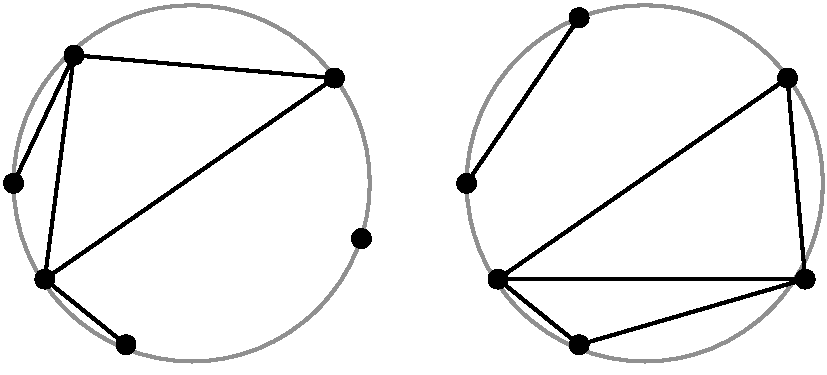
\includegraphics[width=3in]{outerplanar-graphs}}
\vspace{18pt}

Prove that any outerplanar graph is 3-colorable.  A fact you may use 
without proof is that any outerplanar graph has a vertex of degree at 
most 2.

\solution[\newpage]{
Proof by induction on the number of nodes $n$ with the induction 
hypothesis $P(n) =$ ``every outerplanar graph with $n$ vertices is
3-colorable.''

Base case: For $n=1$ the single node graph with no edges is 
trivially outerplanar and 3-colorable.

Inductive step: Assume $P(n)$ holds and let $G_{n+1}$ be an
outerplanar graph with $n+1$ vertices.  There must exist a vertex 
$v$ in $G_{n+1}$ with degree at most 2.  Removing $v$ and all its
incident edges leaves a subgraph $G_n$ with $n$ vertices.

Since $G_{n+1}$ could be drawn with its vertices on a circle and
its edges drawn as straight lines without intersections,
any subgraph can also be drawn in such a way and so $G_n$ is also
an outerplanar graph.  $P(n)$ implies $G_n$ is 3-colorable.  
Therefore we can color all the vertices in $G_{n+1}$ other than $v$
using only 3 colors and since $\deg(v) \leq 2$ we may color it a 
color different than the vertices adjacent to it using only 3 
colors.  Therefore, $G_{n+1}$ is 3-colorable and $P(n+1)$ holds.

}
\end{problem}





%%%%%%%%%%%%%%%%%%%%%%%%%%%%%%%%%%%%%%%%%%%%%%%%%%%%%%%%%%%%%%%%%%%%
\newpage
\begin{problem}{16}
  Consider a stable marriage problem with 4 boys and 4 girls. Here
  are their preference rankings:

\begin{center}
\begin{tabular}{r|c} 
Alfred:    & Grace, Helen, Emily, Fiona    \\
Billy:     & Emily, Grace, Fiona, Helen    \\
Calvin:    & Helen, Emily, Fiona, Grace    \\
David:     & Helen, Grace, Emily, Fiona
\end{tabular}
\end{center}

\begin{center}
\begin{tabular}{r|c} 
Emily:     & Calvin, Alfred, David,  Billy    \\
Fiona:     & Alfred, Billy,  Calvin, David    \\
Grace:     & Alfred, Calvin, David,  Billy    \\
Helen:     & Alfred, Billy,  David,  Calvin
\end{tabular}
\end{center}

\bparts

\ppart{5}
Exhibit a stable matching between the boys and girls.

\solution[\vspace{2in}]{
(Alfred, Grace), (Billy, Fiona), (Calvin, Emily), (David, Helen)
}

\ppart{5} Explain why this is the only stable matching possible.

\solution[\newpage]{
  The Mating Ritual reveals that the boy-optimal and boy-pessimal
  (obtained by switching the roles of boys and girls) matchings are the
  same, so the matching in the previous part is unique.
}

\ppart{6} Suppose that Harry is one of the boys and Alice is one of the girls
when a Mating Ritual is performed.  Circle the properties
below that must be preserved invariants.
\renewcommand{\theenumi}{\roman{enumi}}
\renewcommand{\labelenumi}{(\theenumi)}

\begin{enumerate}

\item Harry is serenading Alice.

% \item Alice is the only girl on Harry's list.

% \item Three girls have boys serenading them.

\item Alice is crossed off Harry's list.

\item Alice likes her favorite better than Harry.

%\item Alice has no suitors.

\item Alice has at least one suitor.

%\item Alice has exactly one suitor.

\item Harry is serenading a girl he likes better than Alice.

\item Harry is serenading a girl he likes less than Alice.


\end{enumerate}

\solution{
\mbox{ }

\begin{enumerate}

\item NOT preserved.  Harry will be rejected when Alice gets a better suitor.

\item Preserved.  No girls ever get added to Harry's list, so if Alice is
  off, she stays off.

\item Preserved: the quality of Alice's favorites is weakly increasing.

\item Preserved: the quality of Alice's favorites is weakly increasing.

\item NOT preserved; if the girl he is serenading rejects him, Alice
  might be next on Harry's list.

\item Preserved: the quality of the girl Harry serenades is is weakly decreasing.

\end{enumerate}
}

\eparts

\end{problem}








\newpage
\begin{problem}{20}

Consider the simple graph $G$ given in Figure $1$.

\begin{figure}[h]
\begin{center}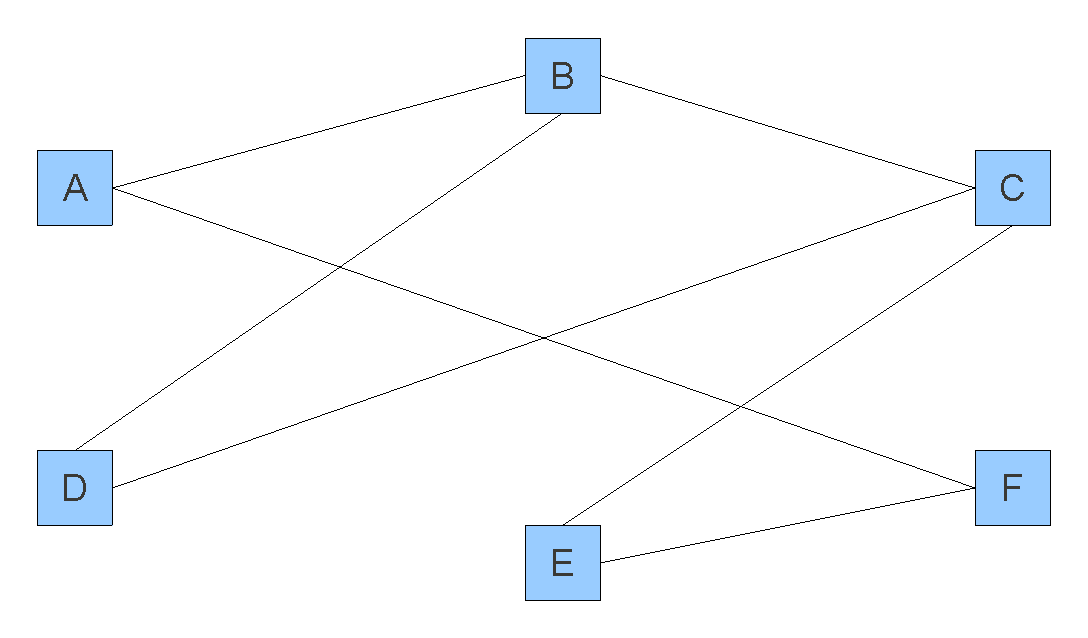
\includegraphics[width=12cm]{unweightedGraph.pdf}\end{center}
\caption{Simple graph G}
\end{figure}

\bparts

\ppart{4}
Give the diameter of $G$.
\solution[\vspace{2in}]{
Recall that the diameter is the maximum of all shortest path lengths between pairs of vertices.  Note that the shortest path length between $D$ and $F$ is $3$, and all other pairs of non-adjacent vertices share a neighbor.
}

\ppart{4}
Give a Hamiltonian Cycle on $G$.
\solution[\vspace{2in}]{
One possible solution is $(A, F, E, C, D, B, A)$.  This cycle and its reverse should constitute all possible solutions.
}

\newpage

\ppart{4}
Give a coloring on $G$ and show that it uses the smallest possible number of colors.
\solution[\vspace{3.5in}]{
One possible $3$-coloring is: $\{A, D, E\}$ red; $\{B, F\}$ green; $C$ blue.  Because there exists an odd-length cycle (e.g. $(B, D, C)$), no $2$-coloring exists.  Therefore the given coloring uses the least possible number of colors. 
}

\ppart{4}
Does $G$ have an Eulerian cycle?  Justify your answer.
\solution[\vspace{2in}]{No.  This follows from the fact that there exist vertices with odd degree; e.g. $B$.}

\eparts

\end{problem}





\newpage
\begin{problem}{18}

    In this problem, we say that an \emph{$M \times N$ grid network} is a
    routing network consisting of an undirected grid of $M$ rows and $N$
    columns, with $M$ inputs on the left and $M$ outputs on the right, as
    depicted in Figure~\ref{3x3grid}. (Note: this is not the same as the ``2-D
    array'' in the notes, which has outputs on the bottom.)
    
\bparts

\ppart{6} What is the congestion of the $3 \times 3$ grid in
Figure~\ref{3x3grid}? (Feel free to use the grids drawn on the next page
in expressing your answer.)

\begin{figure}[h]
    \begin{center}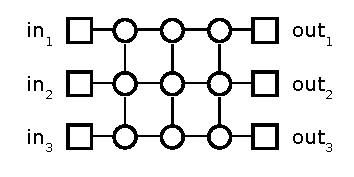
\includegraphics{3x3grid.pdf}\end{center}
    \caption{A $3 \times 3$ grid network.}
    \label{3x3grid}
\end{figure}


\solution[\vspace{5in}]{
    The congestion is 2. We can draw congestion $\leq 2$ routings for all
    six permutations (routing problems), as seen in Figure~\ref{3x3sols}.
    None of these have a congestion 1 solution except for the identity
    permutation; for a rigorous argument see part (b).

    \begin{figure}[h]
        \begin{center}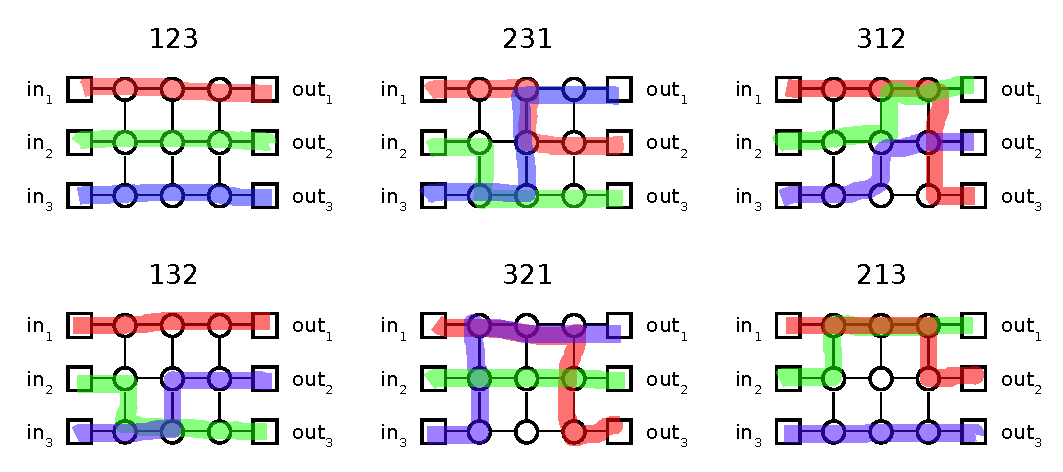
\includegraphics[width=15cm]{3x3sols.pdf}\end{center}
        \caption{Congestion $\leq 2$ routings for part (a).}
        \label{3x3sols}
    \end{figure}

}

\newpage
\begin{figure}[h!]
\begin{center}
    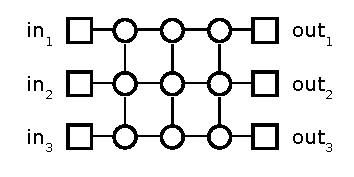
\includegraphics{3x3grid.pdf} \quad
    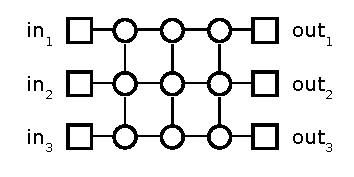
\includegraphics{3x3grid.pdf} \quad \\[1.5em]
    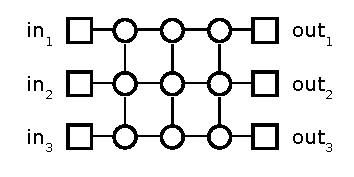
\includegraphics{3x3grid.pdf} \quad
    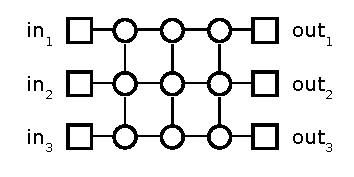
\includegraphics{3x3grid.pdf} \quad \\[1.5em]
    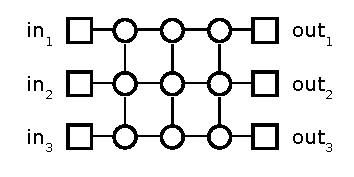
\includegraphics{3x3grid.pdf} \quad
    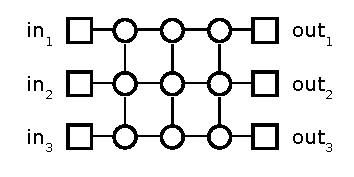
\includegraphics{3x3grid.pdf} \quad \\[1.5em]
    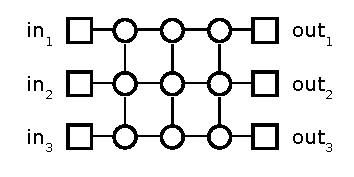
\includegraphics{3x3grid.pdf} \quad
    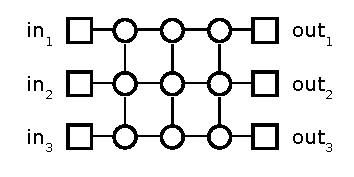
\includegraphics{3x3grid.pdf} \quad \\[1.5em]
    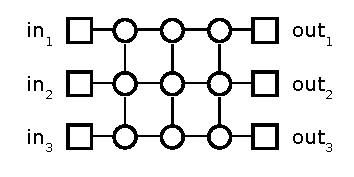
\includegraphics{3x3grid.pdf} \quad
    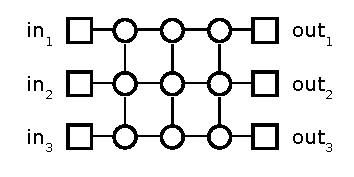
\includegraphics{3x3grid.pdf} \quad \\[1.5em]
    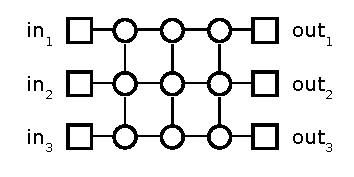
\includegraphics{3x3grid.pdf} \quad
    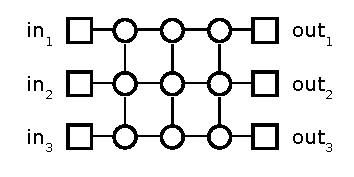
\includegraphics{3x3grid.pdf} \quad
\end{center}
\end{figure}

\newpage
\ppart{6} For the $M \times N$ grid network with $M$ inputs on the left
    and $M$ outputs on the right, prove carefully that the congestion is always
    strictly greater than $1$, so long as $M > 1$.

    \solution[\vspace{6in}]{
        Let $(x,y)$ denote coordinates on the grid, for which $(1,1)$ is the
        upper-left corner and $(M,N)$ is the lower-right corner.

        Consider a congestion $1$ routing on this grid. We show, by strong
        induction on $x$, that for all $1 \leq x \leq N$ and $1 \leq y \leq M$,
        the $x$th step of route $y$ is to move to vertex $(x,y)$. The base case
        of $x=1$ is clear: the switch $(1,y)$ is the only switch connected to 
        $\mathsf{in}_y$, and so the first move is forced. 
        Now in the inductive step, suppose that for all $1 \leq y \leq M$ and
        all $i < x$, the $i$th step of route $y$ was to visit vertex $(i,y)$.
        Then at step $x$, route $y$ can not move up, down, or left on the grid,
        as the vertex there (if any) has already been visited, and congestion
        is constrained to be $1$. So the route must move right to $(x,y)$. This
        completes the induction.

        So any congestion $1$ routing must have each route move right along the
        grid rows until it reaches an output. Then the route starting at
        $\mathsf{in}_i$ can only reach $\mathsf{out}_i$, and for $M > 1$, not
        every routing permutation is possible with congestion $1$.
    }

\newpage
\ppart{6} For the $M \times N$ grid, as in part (b), argue that for any
    $M > 1$, it is possible to choose $N$ large enough so that the grid
    has congestion $2$. (A fully-fledged proof is not required, but give
    justification.)

    \emph{Hint: imagine routes traveling along rows and swapping in
    various places.}

    \solution[\newpage]{
        As in the hint, we imagine routes that travel along rows except
        when participating in a swap move as depicted in
        Figure~\ref{swapmove}.

        \begin{figure}[h]
            \begin{center}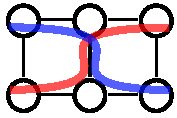
\includegraphics[width=3cm]{swapmove.pdf}\end{center}
            \caption{A swap move with congestion $2$.}
            \label{swapmove}
        \end{figure}

        Any routing of this form has congestion $2$, so it suffices to
        show that we can find such a routing for any given routing
        problem. There are many ways to do this, and some might recognize
        this as the general mathematical fact that sequences of swaps of
        adjacent elements can achieve any permutation. We give a concrete
        approach below.

        We construct the routing from left to right along the grid, adding
        swap moves to move routes between grid rows. As we may assume $N$
        to be as large as necessary, we may apply as many swap moves as
        necessary. Suppose that input $\mathsf{in}_i$ corresponds
        to the bottom output $\mathsf{out}_M$; then we first swap row $i$
        with row $i+1$, then $i+1$ with $i+2$, and so on until the route
        from $\mathsf{in}_i$ leads to row $M$, where it will cease to
        participate in swaps and ultimately lead to output $\mathsf{out}_M$.
        We then do the same for the route destined for $\mathsf{out}_{M-1}$;
        these swaps will not interfere with the bottom-most route. We repeat,
        moving up the line of outputs, until all routes are on the correct
        output row.

        An example is given in Figure~\ref{swapex}, for the following
        permutation of five elements:
        $$ 1 \mapsto 3, \; 2 \mapsto 5,\; 3 \mapsto 4,\; 4 \mapsto 1,\; 5 \mapsto 2. $$

        \begin{figure}[h]
            \begin{center}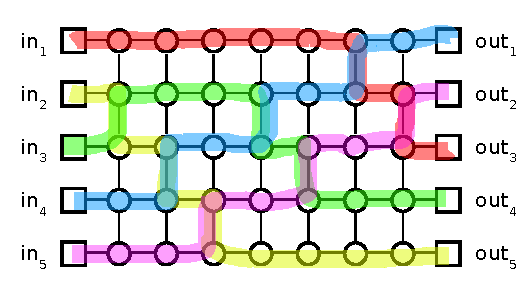
\includegraphics[width=12cm]{swapex.pdf}\end{center}
            \caption{An example routing produced by the solution procedure.}
            \label{swapex}
        \end{figure}
    }

\eparts

\end{problem}





\newpage
\begin{problem}{15}

Throughout this problem, PageRank is understood to mean \emph{unscaled} PageRank.

\bparts

\ppart{5} Given any strongly connected web graph $G$ on at least $2$ vertices, argue that no single vertex can have equilibrium PageRank value greater than $\frac{1}{2}$.

\solution[\vspace{3.5in}]{
    Let $v$ be a vertex with equilibrium value $\lambda$. If we apply the PageRank update step, the PageRank value $\lambda$ at $v$ is distributed to the rest of the graph in some way, and $v$ takes on contributions from the rest of the graph, of total value $\mu \leq 1 - \lambda$. As the PageRank values are in equilibrium, these two are equal; thus: 
$$ \lambda = \mu \leq 1 - \lambda, $$
$$ \lambda \leq \frac12. $$
}


\ppart{5} Let $N \geq 2$ be given. Exhibit a web graph on $N$ vertices in which one vertex has equilibrium PageRank value equal to $\frac{1}{2}$.

\solution[\vspace{3.5in}]{
    Consider the graph consisting of a single hub $H$ and $N-1$ peripheral pages $P_i$ each with a link to and from $H$. Then if we assign the PageRank value $\frac12$ to the hub $H$, and value $\frac{1}{2(N-1)}$ to each page $P_i$, the PageRank values are in equilibrium.
}

\newpage
\ppart{5} Argue that for each $N$, there is only one solution to part (b) that is strongly connected.

\solution[\vspace{3.5in}]{
    In order for a vertex $v$ to have equilibrium PageRank $\frac12$, the inequalities in part (a) must be tight: during the update step, $v$ must take on the entirety of the PageRank from the rest of the graph. This is only possible if every other vertex has an edge to $v$ and has no other outbound edges. This almost entirely determines the graph; the only remaining question concerns the edges out of $v$; but $v$ must have an edge to every other vertex $w$ in order for $w$ to be reachable from $v$, i.e.\ in order for the graph to be strongly connected.
}

\eparts

\end{problem}


%%%%%%%%%%%%%%%%%%%%%%%%%%%%%%%%%%%%%%%%%%%%%%%%%%%%%%%%%%%%%%%%%%%%%%%%%%%%5

\newpage

\begin{problem}{10}
Consider the following relation on the set of natural numbers:
$$R = \{(x,y) : x \leq y^2 \mbox{ for } x, y \in \mathbb N \}.$$
Which of the following properties holds for $R$? If it has the property, prove it. If not, provide a counterexample.

\bparts

\ppart{2} Reflexivity.

\solution[\vspace{2in}]{
Yes.  R is reflexive if $\forall x$ $xRx$, that is, 
if $x \leq x^2$.  If $x = 0, 0 \leq 0,$ so reflexivity holds.  
If $x \geq 1$, then it follows that
$x^2 \geq x$, from multiplying both sides of the inequality by $x$, which is positive.  
This covers all $x \in \mathbb N$.
}

\ppart{2} Symmetry.

\solution[\vspace{2in}]{No.  Counterexample: x = 0, y = 1.  $0 \leq 1^2$, but $1 > 0^2$.}

\ppart{2} Transitivity.

\solution[\vspace{2in}]{No.  Counterexample: $x = 10, y = 5, z = 3$.  $10 \leq 5^2$, 
and $5 \leq 3^2$, but $10 \geq 3^2$.}
\newpage
\ppart{2} Antisymmetry.

\solution[\vspace{2in}]{No.  Counterexample: $x = 2, y = 3$.  
$2 \leq 3^2$, and $3 \leq 2^2$, but $3 \neq 2$.}
\ppart{2} The property of being an equivalence relation.

\solution[\vspace{2in}]{No.  An equivalence relation must 
be reflexive, symmetric, and transitive.  Of those three, the 
relation is only reflexive.}

\eparts

\end{problem}


\end{document}
